\hypertarget{a-formulation-workflow-that-preserves-unresolved-alternatives}{%
\section{A formulation workflow that preserves unresolved
alternatives}\label{a-formulation-workflow-that-preserves-unresolved-alternatives}}

\label{exec13:formulation}

A language model can make a business question more precise by exposing
the decisions that its wording leaves open. Its useful output is a set
of explicit candidate questions, with evidence for their variables and
clocks, followed by a reasoned choice of a supported analysis. Fluency
alone does not determine which candidate the bank intended. A formal
causal engine also cannot repair a mistake that was made before the
graph, intervention and target reached the engine.

Consider a manager who asks, ``Which customers should receive a
retention invitation next month, and how much value will it create?''
One interpretation is the effect of offering the invitation to every
currently eligible customer. Another is the effect among customers who
historically received it. A third is the value of a targeting rule under
a fixed contact budget. The first two are averages over different
populations. The third also requires a feasible policy class, the
information available when the rule acts, a comparator policy and a cost
definition. A model that estimates historical recipients' average effect
and calls it the expected value of the new targeting rule has changed
the question.

The formulation record should therefore contain the eligible population
and exclusions, the sampling unit, invitation and comparator, actual
receipt if distinct, the decision time, permissible information, outcome
horizon, monetary units and accounting treatment of contact cost. It
should distinguish invitation from successful contact and from
subsequent product use. Those variables may be causally related, but
they are different interventions. It should also retain alternatives
that remain unresolved: all eligible customers versus historical
recipients, a single action versus a sequence, and gross revenue versus
net value.

For a binary invitation \(A\), a baseline record \(W\) available at time
zero, and a fixed-horizon outcome \(Y\), an initial target may be

\[
 \psi=\mathbb E_{\nu}\{Y(1)-Y(0)\},
\]

where \(\nu\) names the eligible population. The adjustment expression

\[
 \psi=\int\{m_1(w)-m_0(w)\}\,d\nu(w),
 \qquad m_a(w)=\mathbb E[Y\mid A=a,W=w],
\]

requires consistency, conditional exchangeability, positivity, suitable
sampling and the declared interference restriction. The model may help
elicit and document those assumptions. It cannot infer their truth from
a plausible explanation or from a successful estimator call. In a
generated development example, the project can stipulate and inspect the
complete assignment law. In a later bank application, the assignment
mechanism and measurement meanings need accountable scientific
ownership.

\hypertarget{what-the-frontier-evidence-supports}{%
\subsection{What the frontier evidence
supports}\label{what-the-frontier-evidence-supports}}

The knowledge-assisted perspective of Kıcıman and colleagues motivates
graph drafts, critique and connections to formal tools. Its own
memorization probes and discussion of novel scenarios limit what
benchmark success establishes. The inspected original distinguishes
knowledge-based graph generation from conventional discovery from
observations. For this proposal, a directional suggestion is a
hypothesis with source provenance, not a discovered bank fact. A model
can suggest that financial distress confounds retention contact and
subsequent deposits; the analysis still needs to determine what was
measured, when staff observed it and how it affected assignment.
\citep{v12_la_2305_00050}

The medical co-pilot proposal develops a causal roadmap from a
scientific question through study design and interpretation. Its
examples of prevalent versus incident users are directly relevant to the
distinction between existing account holders and newly eligible
customers. That transfer is a project design proposal, not evidence that
a medical demonstration validates banking workflows. The paper's
evaluation discussion also makes clear that medical question-answering
ability and causal study-design quality are different evaluation
targets. Carefully cued illustrative responses do not establish reliable
autonomous formulation. \citep{v12_la_2407_19118}

CLadder provides formally generated causal questions and explicitly
separates levels of causal reasoning. Its results and limitations
support using a formal reference to evaluate whether verbalized
information was translated into the right query. Binary answer accuracy
on its selected query families does not measure effect calibration,
correct bank populations or decision loss. The paper also identifies the
language-to-formal-tool interface as a remaining problem. The proposed
baseline therefore checks the structured query before it scores a
numerical answer. \citep{v12_la_2312_04350}

The 2026 CausalDS paper adds narrated synthetic structural models, data
files, an observation layer and separate private scoring information. It
distinguishes the conceptual variables used for identification from
their noisy observed proxies. Its reported results separate symbolic
reasoning, estimation, interval quality, abstention and tool cost. This
is useful evidence for a multidimensional evaluation: correctly
extracting a story's graph does not guarantee that the observed data
identify or precisely estimate the stated effect. The paper's historical
model results are author-reported; they have not been reproduced in this
project. \citep{v12_la_2607_08093}

The 2026 observational causal-inference agent paper provides a concrete
principal, actor and critic workflow built around deterministic analysis
tools and reproducible notebooks. It reports favorable comparisons under
its evaluated settings, while its disguised observational-study examples
retain important overlap-related refusals. This supports investigating
constrained analytical workflows with explicit diagnostics. It does not
establish unmeasured-confounding control, longitudinal-policy
identification or valid conditional coverage after the critic selects
which estimates to report. Its point-in-time scope must survive transfer
to the banking proposal. \citep{v12_la_2607_22443}

Two additional primary studies sharpen the boundary between an effective
workflow and causal truth. Sng and colleagues study inconsistencies in
causal-edge ratings and compare retrieval augmentation with a
debate-and-arbiter design. Their retrieval experiment supplies a mocked
true causal graph. The authors explicitly state that reduced
inconsistency does not imply accurate causal prediction and call for
true-graph validation. The title's language about eliminating
hallucinations should therefore not become a guarantee in this product
proposal. Consistent agents can agree on an incorrect edge, and a
retrieval corpus can encode the same incorrect premise.
\citep{exec13_hallucination}

CausalPulse describes query planning, semantic descriptions, process
constraints, agent cards and MCP/A2A coordination for manufacturing
diagnostics. Its reported operational success is a useful architecture
comparison. The paper separately reports root-cause attribution, with a
PSE Hits@1 of 0.44 and F1 of 0.39, using annotations of variables that
changed at the anomaly time. Such annotations and tool-invocation
success are different from interventional causal truth. The paper's
local timing setup and manufacturing deployment discussion likewise do
not establish banking runtime or treatment-effect performance. We can
adapt its separation of semantic services, deterministic tools and
workflow state as a design pattern while retaining those scientific
limits. \citep{exec13_pulse}

These studies suggest complementary roles: retrieve definitions, draft
alternatives, check logical consistency, construct typed calls, retain
execution artifacts and explain formal results. The adverse findings
point to the same missing link: a linguistic interpretation must be
checked against the intended population, intervention, measurement model
and information clock. An additional critic can help find mistakes, but
agreement between related models is not independent validation of an
assumption.

\hypertarget{a-worked-failure-an-overlap-remedy-changes-the-population}{%
\subsection{A worked failure: an overlap remedy changes the
population}\label{a-worked-failure-an-overlap-remedy-changes-the-population}}

Suppose the bank initially asks for the average invitation effect among
all eligible customers. A diagnostic finds weak overlap for one customer
stratum. An agent proposes trimming that stratum and continues to report
the result as if it answered the original question. Even with perfect
estimation, that continuation can be wrong.

To isolate the target issue, stipulate a three-stratum population with
known masses, propensities and conditional effects. These are generated
numerical assumptions; the units of the conditional effect are thousands
of currency units per customer.

\begin{longtable}[]{@{}>{\raggedright\arraybackslash}p{\dimexpr 0.15\linewidth-2\tabcolsep\relax}>{\raggedright\arraybackslash}p{\dimexpr 0.5\linewidth-2\tabcolsep\relax}>{\raggedright\arraybackslash}p{\dimexpr 0.35\linewidth-2\tabcolsep\relax}@{}}
\toprule
\begin{minipage}[b]{\linewidth}\raggedright
Stratum \(w\)\strut
\end{minipage} & \begin{minipage}[b]{\linewidth}\raggedright
Population mass \(p(w)\), invitation propensity \(e(w)\)\strut
\end{minipage} & \begin{minipage}[b]{\linewidth}\raggedright
Conditional effect \(\tau(w)\)\strut
\end{minipage}\tabularnewline
\midrule
\endhead
\begin{minipage}[t]{\linewidth}\raggedright
0\strut
\end{minipage} & \begin{minipage}[t]{\linewidth}\raggedright
\(0.5,\ 0.05\)\strut
\end{minipage} & \begin{minipage}[t]{\linewidth}\raggedright
\(0\)\strut
\end{minipage}\tabularnewline
\begin{minipage}[t]{\linewidth}\raggedright
1\strut
\end{minipage} & \begin{minipage}[t]{\linewidth}\raggedright
\(0.3,\ 0.50\)\strut
\end{minipage} & \begin{minipage}[t]{\linewidth}\raggedright
\(2\)\strut
\end{minipage}\tabularnewline
\begin{minipage}[t]{\linewidth}\raggedright
2\strut
\end{minipage} & \begin{minipage}[t]{\linewidth}\raggedright
\(0.2,\ 0.80\)\strut
\end{minipage} & \begin{minipage}[t]{\linewidth}\raggedright
\(8\)\strut
\end{minipage}\tabularnewline
\bottomrule
\end{longtable}

The full-population ATE is \(0.5(0)+0.3(2)+0.2(8)=2.2\). Trimming to
true propensities in \([0.1,0.9]\) retains half the population and gives
\(2.2/0.5=4.4\). The conventional overlap-weighted target instead uses
the measure proportional to \(p(w)e(w)\{1-e(w)\}\):

\[
 \psi_{\rm OW}
 =\frac{\sum_w p(w)e(w)\{1-e(w)\}\tau(w)}
        {\sum_w p(w)e(w)\{1-e(w)\}}
 =\frac{0.406}{0.13075}
 =\frac{1624}{523}\simeq 3.1052.
\]

The effect among treated customers is different again:
\(\psi_{\rm ATT}=316/67\simeq4.7164\). Exact rational calculations
reproduce all four values. None is an empirical estimate from a package
or a live language model. Their disagreement arises entirely from the
population measure. \citep{exec13_formulation_targets}

This distinction is visible in a real proposed reuse path. The inspected
oci-agent notebook applies a propensity-based keep mask and averages
AIPW pseudo-outcomes over that subset while labeling the output ``ATO.''
The accompanying paper describes the trimming remedy in the same
terminology. A hard-trimmed average and an \(e(W)\{1-e(W)\}\)-weighted
overlap effect are not generally equal. The integration must either
label the result as a trimmed-population ATE, with its actual
eligibility rule, or implement and validate the intended weighting
operation. It must also retain the original all-eligible request and the
excluded population. Estimated propensities add randomness to selection;
the simple known-law calculation above does not validate that further
inference step. \citep{v12_la_package_oci_agent,v12_la_2607_22443}

The correct translation response is therefore a revised analysis
proposal: the original target is unresolved under the current
information or diagnostics; a specified restricted-population target may
be feasible; and the bank must assess whether that restricted target
still informs its decision. In a public or generated prototype, this
branch can be evaluated without bank data by stipulating both
populations and checking that the system preserves their difference. It
is not necessary to obtain expensive authentic evidence merely to detect
a target substitution.

\hypertarget{concrete-package-choices-and-the-formal-baseline}{%
\subsection{Concrete package choices and the formal
baseline}\label{concrete-package-choices-and-the-formal-baseline}}

The inspected pywhy-llm path is a candidate for eliciting hypotheses and
candidate variables. Its
\texttt{IdentificationSuggester.suggest\_backdoor} delegates to a
language-model confounder suggester. That class's front-door method is a
stub, whereas \texttt{SimpleIdentificationSuggester} has a front-door
method that generates text suggestions. Neither fact establishes a
formal identification algorithm. The proposal should reuse the
suggestion pattern selectively and send the resulting explicit graph and
query to a separately admitted causal engine. It should preserve cited
source passages and unresolved alternatives instead of interpreting a
generated factor list as an approved adjustment set.
\citep{v12_la_package_pywhy_llm}

For oci-agent, the useful candidate is the separation of a
specification, a deterministic analysis notebook and a critic report.
The selected source has a general notebook runner and a target-label
issue requiring correction. A bounded banking interface should expose
fixed reviewed operations with resource limits and typed outputs. The
proposal does not adopt a general notebook executor as the causal MCP
surface. Dependency resolution, failure handling and executable parity
remain separate implementation tasks; the source's research status is
not a reason to infer a deployed bank service.
\citep{v12_la_package_oci_agent}

CausalDS is a candidate for generated scene and task design, but its
grader needs a semantic review before direct adoption. The inspected
identification/scoring helpers distinguish several genuine states, yet
some missing metadata defaults and finite-interval checks require
attention. Unknown identification due to a missing backend is not
scientific nonidentification. A malformed answer is not a justified
abstention. A capped score can conceal severe tail losses unless the
uncapped losses and coverage are also reported. The proposal therefore
takes the task separation and private-reference design while requiring
explicit metadata and failure validation.
\citep{v12_la_package_causalds}

The deterministic formulation baseline has three layers. A schema check
verifies that population, unit, intervention, comparator, horizon, clock
and scale are present. A semantic check compares these fields with the
supplied brief and dictionary: a post-contact duration cannot become a
pre-contact covariate, an invitation cannot silently become actual
uptake, and a requested all-eligible effect cannot become a
recipients-only effect. A formal check evaluates identification under
the explicitly supplied candidate graph and returns an expression,
model-relative nonidentification, unsupported scope or an unresolved
input. These checks validate different things. A well-formed schema does
not prove the story is true, and a correctly evaluated graph does not
prove its edges.

For a generated benchmark, the reference can enumerate a finite set of
admissible formulations \(\mathcal Q(b)\) for brief \(b\). An explicitly
resolved brief may have one acceptable target. An ambiguous brief may
have several and require the system to request or retain the missing
distinction. A baseline can return those alternatives directly from the
supplied reference fields and use exact calculations such as the example
above. This establishes a transparent lower-cost comparator and exposes
what a language model is expected to add: interpretation of unstructured
language, evidence retrieval and useful clarification, rather than
numerical work already handled by a deterministic engine.

\subsection{A convincing explanation is not yet an intervention estimate}
\label{closure30:formulation}

A corporate borrower says that a tight credit line prevents it from accepting
an overseas order. A language assistant may recover the relevant passage,
connect it to the financial statements and explain why working capital matters.
The lender still faces a different question: how would a specified change in
credit terms affect exports, repayment and contribution? The answer depends on
why the borrower faces the constraint and what the proposed facility changes.
Good extraction is useful evidence preparation. It does not supply the missing
comparison between alternative lending decisions.

\subsubsection{What the financing-and-exports study actually measures}

Li's September 2025 preprint is directly relevant to this distinction. Its
proposed procedure first extracts financing constraints, then export outcomes,
and finally asks a language model to explain a mechanism using economic
theories. The first extraction records a constraint, its severity, supporting
evidence and type. The second records an export metric, value, description and
direction. These explicit intermediate records would help an analyst challenge
an unsupported interpretation of a company report. Equations (1)--(10) define
the information passed between these stages. \citep[Sections 3.1--3.4]{rel18li}

The reported Financing-Export Dataset contains 2,000 Chinese listed firms
over 2015--2019, combining accounts, trade information and text. The stated
comparison uses the same inputs for the proposed prompts and model baselines.
It evaluates financing-constraint classification, subsequent export
participation prediction, repeated-answer consistency and economic relevance
scored by experts. Table~\ref{closure30:exports} reproduces the two rows needed
to understand the claimed improvement; these are the author's reported
scores, not an independently reproduced experiment.

\begin{table}[htbp]
\centering\small
\begin{tabular}{lrrrr}
\toprule
Method & Constraint F1 & Export accuracy & Consistency & Relevance\\
\midrule
Baseline prompts & 0.82 & 76.8\% & 0.78 & 4.1/5\\
Proposed staged prompts & 0.84 & 78.5\% & 0.81 & 4.4/5\\
\bottomrule
\end{tabular}
\caption{Selected reported results from Li's Table 1. The first two columns
measure classification and prediction. Consistency measures repeated outputs;
relevance is an expert assessment of the explanation. None is an estimated
effect of a lending intervention.}
\label{closure30:exports}
\end{table}

The ablation is revealing. Removing the explicit economic-theory guidance
leaves reported F1 and export accuracy at 0.84 and 78.5\%, while consistency
falls to 0.77 and relevance to 3.8/5. This supports the narrower reported
comparison that the guidance changes explanation scores in that experiment.
It does not show that an intervention contrast becomes identified. The
relevance criterion explicitly rewards alignment with economic theory, so
improvement on it is not independent confirmation of the proposed mechanism.
\citep[Sections 4.2.2--4.6; Tables 1--2]{rel18li}

Sections 3 and 4 do not state a treatment-assignment design, a structural
restriction identifying a specified lending effect, or an estimator and
uncertainty interval for that effect. They also do not provide sufficient
model-version, prompt, partition and uncertainty detail to reconstruct the
reported score differences from the paper alone. Those limitations restrict
the use of the evidence; they do not establish that the reported scores are
false. The useful proposal role is a candidate for extracting financial
evidence and developing hypotheses, to be compared on tasks with independently
checked records. Its explanation score cannot value a credit facility.

\subsubsection{The same observed story can imply different lending effects}

Consider a deliberately small model in which $F=1$ denotes a financing
constraint and $Y=1$ denotes export participation. Both are binary. For the
moment, suppose every company report states $F$ and $Y$ perfectly, and an
assistant extracts them without error. This assumption gives the assistant
the best possible measurement of these two variables. It lets us isolate the
identification problem from a language model's mistakes.

In the first explanation, an unobserved distress state $U$ causes both the
constraint and the export outcome. Let $U$ be Bernoulli with probability
$1/2$, and let independent errors $E_F,E_Y$ each be Bernoulli with probability
$1/5$. All three inputs are mutually independent. Define
\begin{equation}
 F=U\mathbin{\oplus}E_F,\qquad
 Y=(1-U)\mathbin{\oplus}E_Y,
 \label{closure30:confounded}
\end{equation}
where $\oplus$ is exclusive-or: it flips a binary value when the error is one.
Distress makes the constraint more likely and participation less likely.
Changing $F$ alone leaves the equation for $Y$ unchanged. In this model,
\begin{equation}
 \Pr\{Y=1\mid\doop(F=0)\}
 =\Pr\{Y=1\mid\doop(F=1)\}=\frac12.
 \label{closure30:noeffect}
\end{equation}

The observed contrast nevertheless looks substantial. Symmetry gives
$\Pr(F=1)=1/2$ and $\Pr(U=1\mid F=1)=4/5$. Consequently,
\begin{align}
 \Pr(Y=1\mid F=1)
 &=\frac45\frac15+\frac15\frac45=\frac8{25},\\
 \Pr(Y=1\mid F=0)
 &=\frac45\frac45+\frac15\frac15=\frac{17}{25}.
\end{align}
The participation difference between constrained and unconstrained firms is
$-9/25$, or minus 36 percentage points, even though the intervention effect
is zero. It reflects the unobserved distress composition of the groups.

In the second explanation, financing itself changes participation. Let
$Z$ be Bernoulli with probability $1/2$ and $E$ independently Bernoulli with
probability $8/25$, and set
\begin{equation}
 F=Z,\qquad Y=(1-F)\mathbin{\oplus}E.
 \label{closure30:causal}
\end{equation}
Now the conditional and interventional risks coincide: they are $17/25$
under $F=0$ and $8/25$ under $F=1$. Removing the constraint raises participation
by $9/25$. Both explanations generate exactly the same table of observations:
\begin{center}
\begin{tabular}{crr}
\toprule
 & $Y=0$ & $Y=1$\\
\midrule
$F=0$ & $4/25$ & $17/50$\\
$F=1$ & $17/50$ & $4/25$\\
\bottomrule
\end{tabular}
\end{center}
Each row sums to $1/2$. Exact enumeration of the independent binary inputs
agrees with these algebraic probabilities and with both intervention
calculations. The constants are stipulated for the example; none is an
estimate for Chinese firms or a bank portfolio. \citep{rel18witness}

\begin{figure}[htbp]
\centering
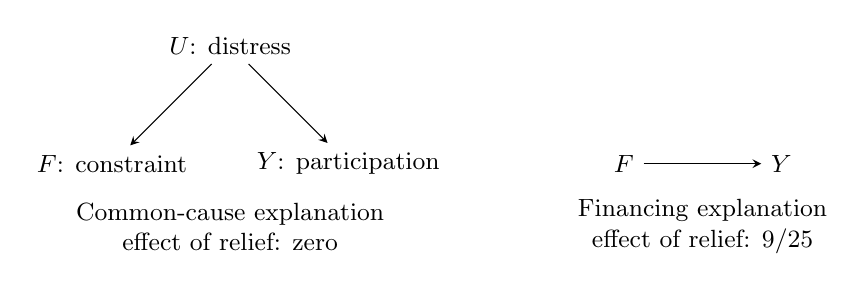
\begin{tikzpicture}[>=stealth,every node/.style={font=\small}]
\node (u) at (0,1.5) {$U$: distress};
\node (f) at (-1.5,0) {$F$: constraint};
\node (y) at (1.5,0) {$Y$: participation};
\draw[->] (u)--(f);\draw[->] (u)--(y);
\node[align=center] at (0,-0.8) {Common-cause explanation\\effect of relief: zero};
\node (f2) at (5,0) {$F$};\node (y2) at (7,0) {$Y$};
\draw[->] (f2)--(y2);
\node[align=center] at (6,-0.8) {Financing explanation\\effect of relief: $9/25$};
\end{tikzpicture}
\caption{The two constructed mechanisms share the observed distribution
of financing constraints and export participation. A report containing only
these facts cannot distinguish their intervention effects.}
\label{closure30:twoworlds}
\end{figure}

Suppose the report is a deterministic transcript $T=t(F,Y)$, recording those
two facts with their values and dates. Then
\begin{equation}
 \Pr(F=f,Y=y,T=t)=\Pr(F=f,Y=y)\,\ind\{t=t(f,y)\}
\end{equation}
is identical in the two explanations. Any fixed extraction or prediction rule
using that information has the same observable performance in both. Random
prompt variation independent of the firm adds no distinction between the two
observational laws. Even an always-consistent explanation can therefore be
attached to two different intervention answers.

Real reports may contain additional information about distress, assignment
or mechanisms. The construction does not exclude that possibility. Such
information must be established and incorporated into the model; a score for
the fluency or plausibility of the resulting explanation cannot substitute
for it. The two effects displayed here demonstrate nonidentification in this
example, not sharp bounds over every compatible causal model.

\subsubsection{Knowledge claims need a task-specific test}

Mugleston and colleagues discuss a broader philosophical question: whether
the internal representations of a language model deserve to be called
knowledge. Their argument considers justified true belief, compressed
representations, contextual understanding and the limitations of the Chinese
room analogy. Section 5 also distinguishes informative coherence from merely
repeating an answer, and Section 9 leaves important claims about understanding
unsettled. The paper describes its purpose as a thought experiment.
\citep[Sections 3.3--6 and 9]{rel18mugleston}

That discussion is relevant to how an analyst interprets assistance, but it
does not resolve a lending estimand. A system can organize useful knowledge
without knowing which of the two mechanisms in Figure~\ref{closure30:twoworlds}
generated a particular dataset. Conversely, calling the system a statistical
text generator does not establish that a specific extracted passage is wrong.
The practical assessment concerns the record, the proposed causal restriction
and the decision that follows from it. Philosophical labels cannot replace
those checks.

For a credit decision, the first commitment is an action the lender can carry
out: for example, an offer with specified limit, maturity, price and eligibility
at a fixed date. Setting an abstract constraint indicator to zero is not
automatically that offer. Take-up, competing lenders, borrower responses and
the cost of capital can intervene between the offer and exports. The target
may concern an offered facility, the facility actually drawn, or net
contribution after expected losses. Those quantities require distinct
comparisons.

A useful assisted study would retain the quoted passages and dates, distinguish
the lender's action from the borrower's condition, and set out alternative
causal explanations. An analyst could then defend additional measurements,
a suitable experiment or a credible source of assignment variation. The
evaluation should score faithful extraction, correct formulation and justified
uncertainty separately. A strong extraction score is valuable on its own;
the effect estimate becomes valuable only when its identification and financial
interpretation are also supported.

\hypertarget{evaluation-before-a-costly-bank-study}{%
\subsection{Evaluation before a costly bank
study}\label{evaluation-before-a-costly-bank-study}}

The initial evaluation can use public data dictionaries and openly
documented financial examples alongside generated causal mechanisms.
Public data support questions about available variables and clocks; they
usually do not supply intervention truth. Generated mechanisms can
supply that truth for the declared model. A reference author should
create matched examples that vary one decisive feature: invitation
versus uptake, all eligible versus treated population, pre-decision
versus post-decision measurement, complete variables versus noisy
proxies, or a single action versus repeated treatment. The target-change
example supplies one exact reference family. This is a proposed
evaluation design; it is not a reported live-agent comparison.

Train/development and final evaluation should be split by the underlying
scenario or structural model, not merely by paraphrases of the same
question. Otherwise a system can learn the reference target from exposed
near-duplicates. All requests should remain in the evaluation
denominator, including ambiguous requests, timeouts, unsupported
estimands, malformed answers and justified nonidentification. Report
target and clock fidelity, unjustified resolution of ambiguity, false
causal answers, valid abstention, numerical error where a target is
actually identified, interval availability and coverage where ground
truth permits them, and total resource use. A high completion rate alone
rewards an agent for confidently answering questions that should remain
unresolved.

Retrieval, structured prompting and an actor/critic loop should be
compared against the same deterministic baseline and fixed task
families. A retrieval ablation tests whether source passages improve
interpretation. A critic ablation tests whether additional review
catches errors, while reporting the added calls, time and newly
introduced mistakes. A graph-perturbation comparison tests whether a
system notices that an assumption changed. Repeated runs reveal
stability. These studies need their actual model, tool, prompt, data and
stopping-rule identities frozen before final evaluation. Agreement
across repeated runs is useful evidence about stability; it is not
evidence that the agreed answer is causally correct.

Several gaps remain scientific. A general method for recovering
stakeholder intent from incomplete language is not established. The
immediate remedy is to preserve admissible alternatives and make the
missing decision explicit. A general guarantee that retrieval or debate
validates causal edges is also absent; the current studies justify
investigating those tools with factual and graph-specific references,
not treating consensus as truth. Identification from noisy proxies,
dependent observations or repeated interventions requires the
corresponding statistical model and method. Finally, whether an assisted
workflow saves bank analyst time or changes an investment decision
requires a later workflow study after a bounded prototype shows merit.
Those gaps narrow the claims and motivate specific experiments; they do
not prevent writing or testing the proposal's public/generated
formulation contract. The next two studies develop decisions within that
contract: which population or weight class the result protects, and how a
clarification workflow resolves a symbolic goal before selecting tools.
Neither statistical robustness nor goal completion can replace an explicit
choice of the intended causal question. \label{exec13:formulation-end}
